\documentclass{standalone}
\usepackage{tikz,pgfplots}
\pgfplotsset{compat=newest}
\begin{document}

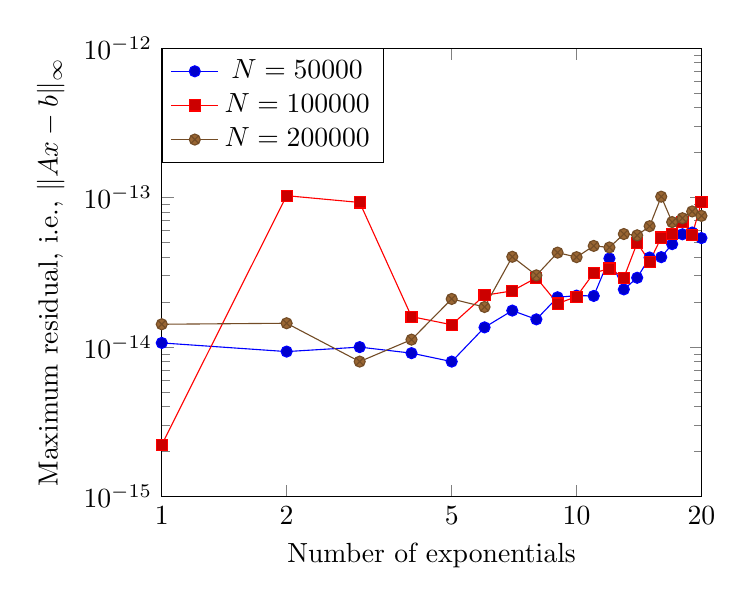
\begin{tikzpicture}
\begin{loglogaxis}[
	xlabel={Number of exponentials},
	ylabel={Maximum residual, i.e., $\Vert Ax-b\Vert_{\infty}$},
	xmin=1, xmax=20,
	ymin=1e-15, ymax=1e-12,
%	log x ticks with fixed point,
	xticklabel style={/pgf/number format/.cd,fixed,precision=2},
    xticklabel={%
      \pgfmathfloatparsenumber{\tick}%
      \pgfmathfloatexp{\pgfmathresult}%
      \pgfmathprintnumber{\pgfmathresult}%
	  },
	  xtick={1, 2, 5,  10, 20},
	  legend style={
	  	at={(0.0,1.0)},
		anchor=north west},
%	xticklabel=\pgfmathparse{10^\tick}\pgfmathprintnumber{\pgfmathresult}
]
%Fast N=50000
\addplot
coordinates{
(1, 1.06581e-14) (2, 9.32587e-15) (3, 9.99201e-15) (4, 9.10383e-15) (5, 7.99361e-15) (6, 1.35447e-14) (7, 1.75415e-14) (8, 1.53211e-14) (9, 2.15383e-14) (10, 2.20934e-14) (11, 2.19824e-14) (12, 3.91909e-14) (13, 2.43139e-14) (14, 2.90878e-14) (15, 3.9746e-14) (16, 3.9968e-14) (17, 4.88498e-14) (18, 5.68434e-14) (19, 5.83977e-14) (20, 5.36238e-14) 
};
\addlegendentry{$N=50000$}
%Fast N=100000
\addplot
coordinates{
(1, 2.22045e-15) (2, 1.03029e-13) (3, 9.28146e-14) (4, 1.59872e-14) (5, 1.40998e-14) (6, 2.22045e-14) (7, 2.37588e-14) (8, 2.90878e-14) (9, 1.95399e-14) (10, 2.17604e-14) (11, 3.13083e-14) (12, 3.35287e-14) (13, 2.90878e-14) (14, 4.9738e-14) (15, 3.73035e-14) (16, 5.40679e-14) (17, 5.68434e-14) (18, 6.86118e-14) (19, 5.62883e-14) (20, 9.30367e-14) 
};
\addlegendentry{$N=100000$}
%Fast N=200000
\addplot
coordinates{
(1, 1.42109e-14) (2, 1.44329e-14) (3, 7.99361e-15) (4, 1.12133e-14) (5, 2.09832e-14) (6, 1.85407e-14) (7, 4.01901e-14) (8, 3.01981e-14) (9, 4.28546e-14) (10, 3.9968e-14) (11, 4.75175e-14) (12, 4.64073e-14) (13, 5.70655e-14) (14, 5.59552e-14) (15, 6.43929e-14) (16, 1.01474e-13) (17, 6.86118e-14) (18, 7.28306e-14) (19, 8.08242e-14) (20, 7.54952e-14) 
};
\addlegendentry{$N=200000$}
\end{loglogaxis}
\end{tikzpicture}
\end{document}